\documentclass[12pt,a4paper]{article}

% Pacotes básicos
\usepackage[utf8]{inputenc}
\usepackage[T1]{fontenc}
\usepackage[brazil]{babel}
\usepackage{graphicx}
\usepackage{float}
\usepackage{amsmath, amssymb}
\usepackage{hyperref}
\usepackage{caption}
\usepackage{cite}
\usepackage{listings} % para formatar blocos de código
\usepackage{enumitem} % para controlar listas
\usepackage{xcolor}   % necessário para cores no listings

\usepackage{multirow}
\usepackage{array}
\usepackage{booktabs}
\usepackage{colortbl}  % for \cellcolor command

\begin{document}

% Configurações do listings
\lstset{
  language=Python,
  basicstyle=\ttfamily\small,
  numbers=left,
  numberstyle=\tiny,
  frame=single,
  breaklines=true,
  keywordstyle=\color{blue}\bfseries,
  stringstyle=\color{red},
  commentstyle=\color{green!60!black}\itshape,
  showstringspaces=false
}

\graphicspath{{../img/}}


% ==============================
% CAPA
% ==============================
\begin{titlepage}
    \centering
    {\Large \textbf{Universidade Federal de Minas Gerais}}\\[0.3cm]
    {\large Engenharia de Sistemas}\\[2cm]

    {\Huge \textbf{NS3: formando topologias básicas}}\\[1.5cm]

    \textbf{Introdução a sistemas computacionais}\\[0.5cm]
    \textbf{Professor: Aldri Luiz dos Santos}\\[1.5cm]
    
    \begin{flushleft}
        \textbf{Aluno:}\\
        Josoé Santos Queiroz --- 2019026982
    \end{flushleft}
    
    \vfill
    {\large Belo Horizonte, MG}\\
    {\large \today}
\end{titlepage}

\clearpage
\tableofcontents
\clearpage

% ==============================
% INTRODUÇÃO
% ==============================
\section{Introdução}

NS3 é um simulador de rede discreto, amplamente utilizado para pesquisa e desenvolvimento em redes de computadores. Ele oferece uma plataforma flexível para modelar, simular e analisar o comportamento de redes complexas, auxiliando a simulação de novas ideias e de novas soluções de rede feitas por pesquisadores e engenheiros.

Este relatório descreve a implementação de topologias básicas utilizando o NS3, incluindo a configuração de nós, enlaces e protocolos de comunicação. Com o objetivo de fornecer uma compreensão prática do funcionamento do NS3 e de redes de  computadores. O procedimento deste relatório segue as etapas de instalação, configuração e execução de simulações sugeridas pelo tutorial oficial do NS3 \cite{ns3_tutorial}. Além disso o código fonte escrito, os resultados de simulação e a fonte deste artigo em latex estão disponíveis no repositório GitHub \cite{tp1_repo}.

\section{Ambiente de simulação}

Este relatório descreve a implementação de topologias básicas utilizando o NS3. Os experimentos foram conduzidos em um ambiente MacOS com um processador Apple M4 pro, 16GB de RAM. O NS3 foi instalado e configurado conforme as instruções oficiais disponíveis na documentação do NS3. A figura \ref{fig:ns3_setup} ilustra a configuração do ambiente de simulação. Note que a configuração foi feita com sucesso porque a IDE reconheceu as classes do NS3 e não acusou erro no código fonte.

\begin{figure}[H]
    \centering
    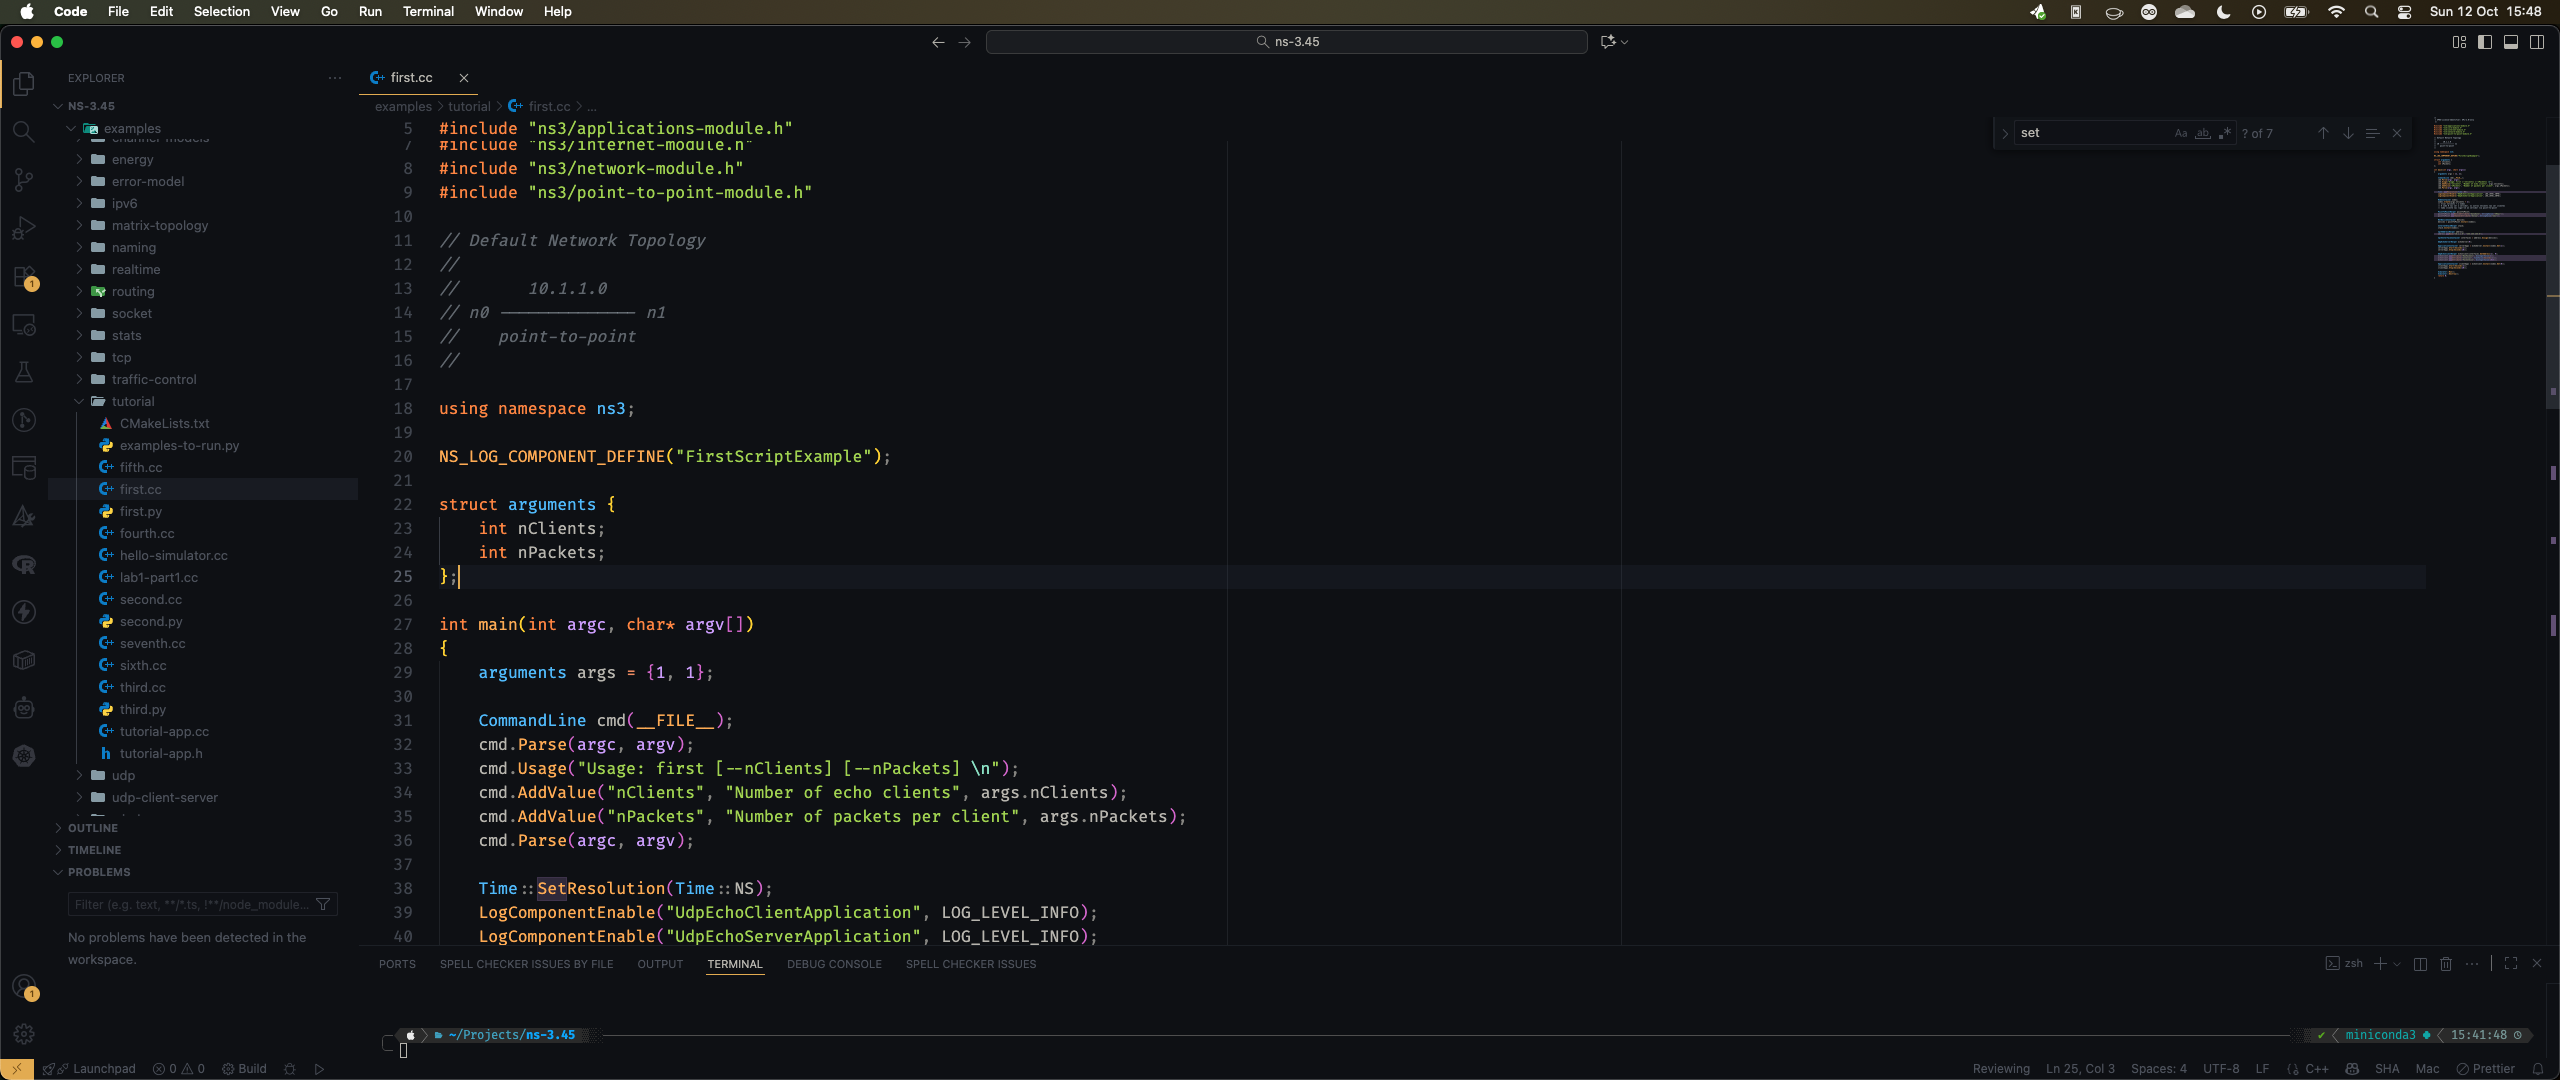
\includegraphics[width=1\textwidth]{initial_setup.png}
    \caption{Configuração do ambiente de simulação NS3}
    \label{fig:ns3_setup}
\end{figure}

A figura \ref{fig:ns3_test} mostra o resultado da execução dos testes que verificam se a instalação do NS3 foi bem sucedida. Todos os testes foram concluídos com sucesso, indicando que o ambiente está pronto para o desenvolvimento do trabalho.

\begin{figure}[H]
    \centering
    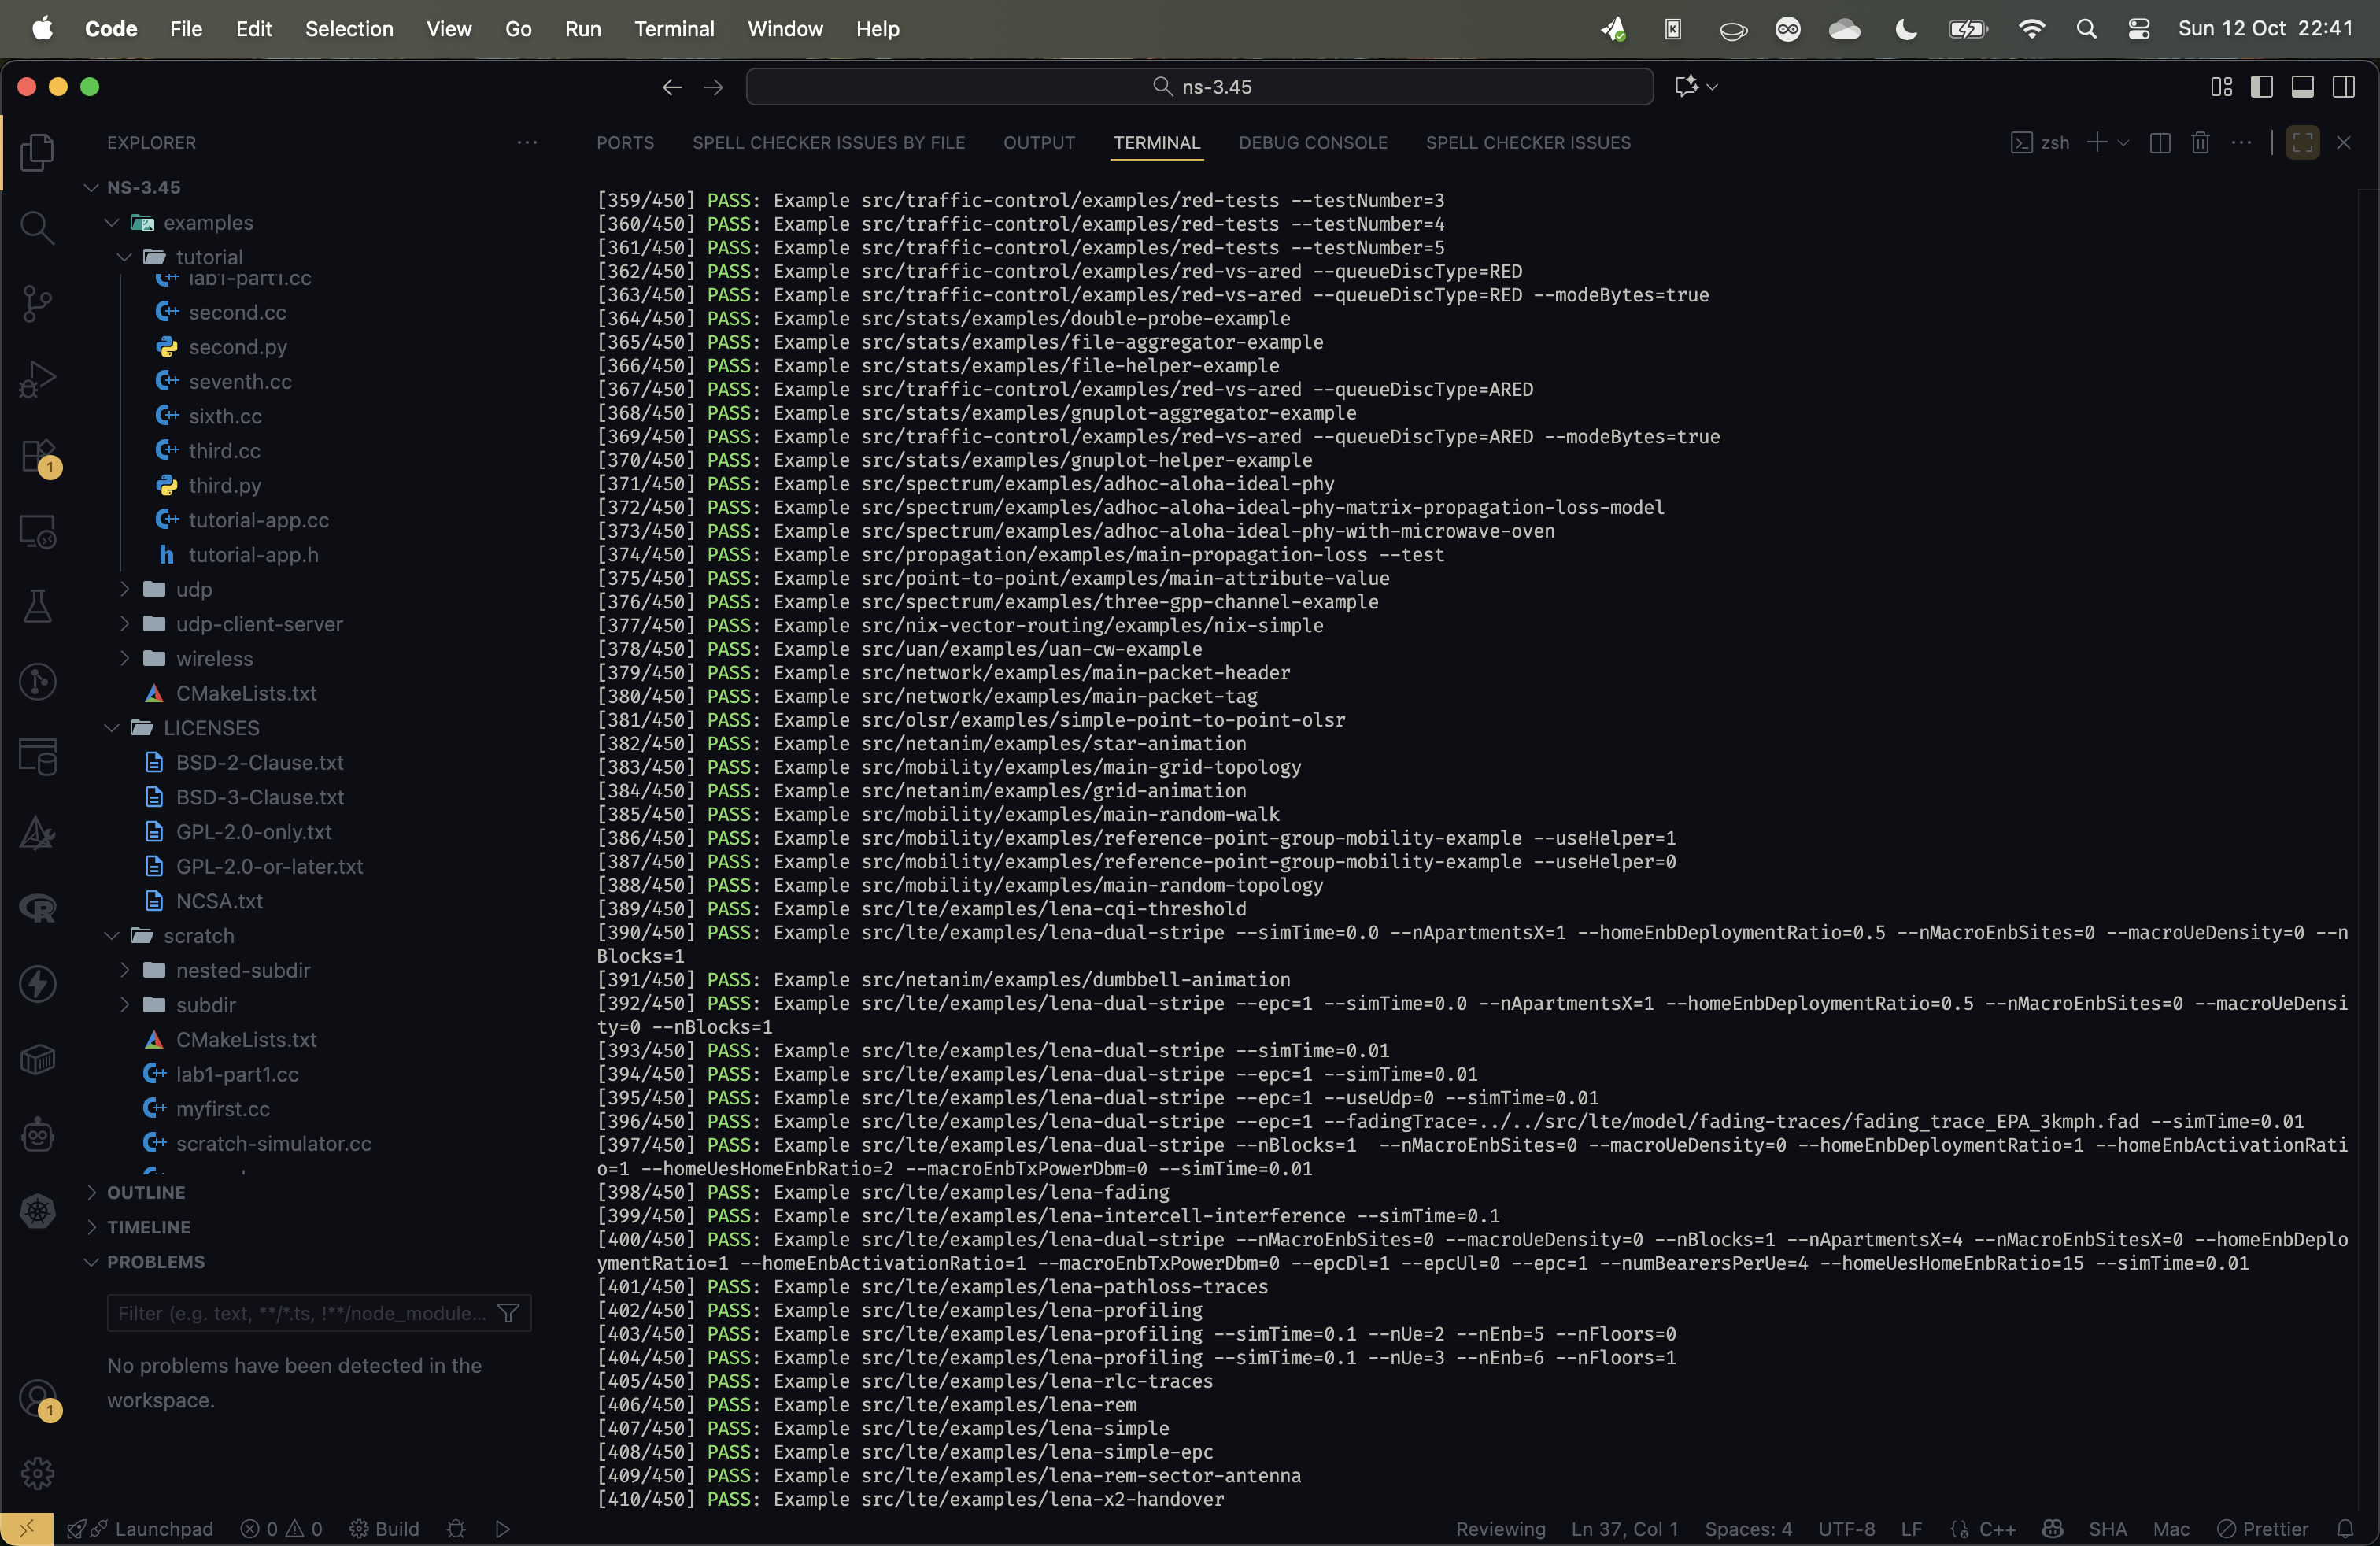
\includegraphics[width=1\textwidth]{test_results.png}
    \caption{Resultados dos testes de instalação do NS3}
    \label{fig:ns3_test}
\end{figure}

\section{Simulações}

\subsection{Topologia em estrela}

A primeira topologia implementada foi a topologia em estrela, onde um nó central se conecta a vários nós periféricos. A figura \ref{fig:star_topology_layout} ilustra a configuração dessa topologia. Nesta configuração o centro da estrela é um servidor com endereço IP 10.1.1.1 que se conecta aos clientes em outras subredes.

\begin{figure}[H]
    \centering
    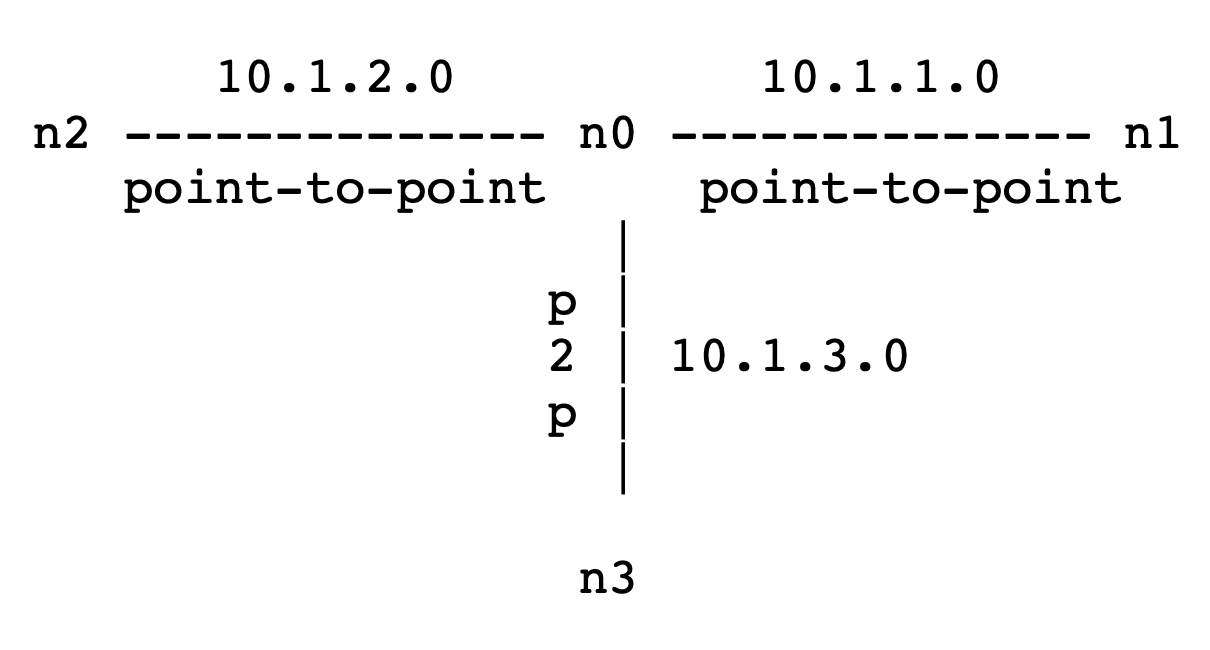
\includegraphics[width=1\textwidth]{star_topology.png}
    \caption{Topologia em estrela com 3 clientes e 1 servidor.}
    \label{fig:star_topology_layout}
\end{figure}


\begin{figure}[H]
    \centering
    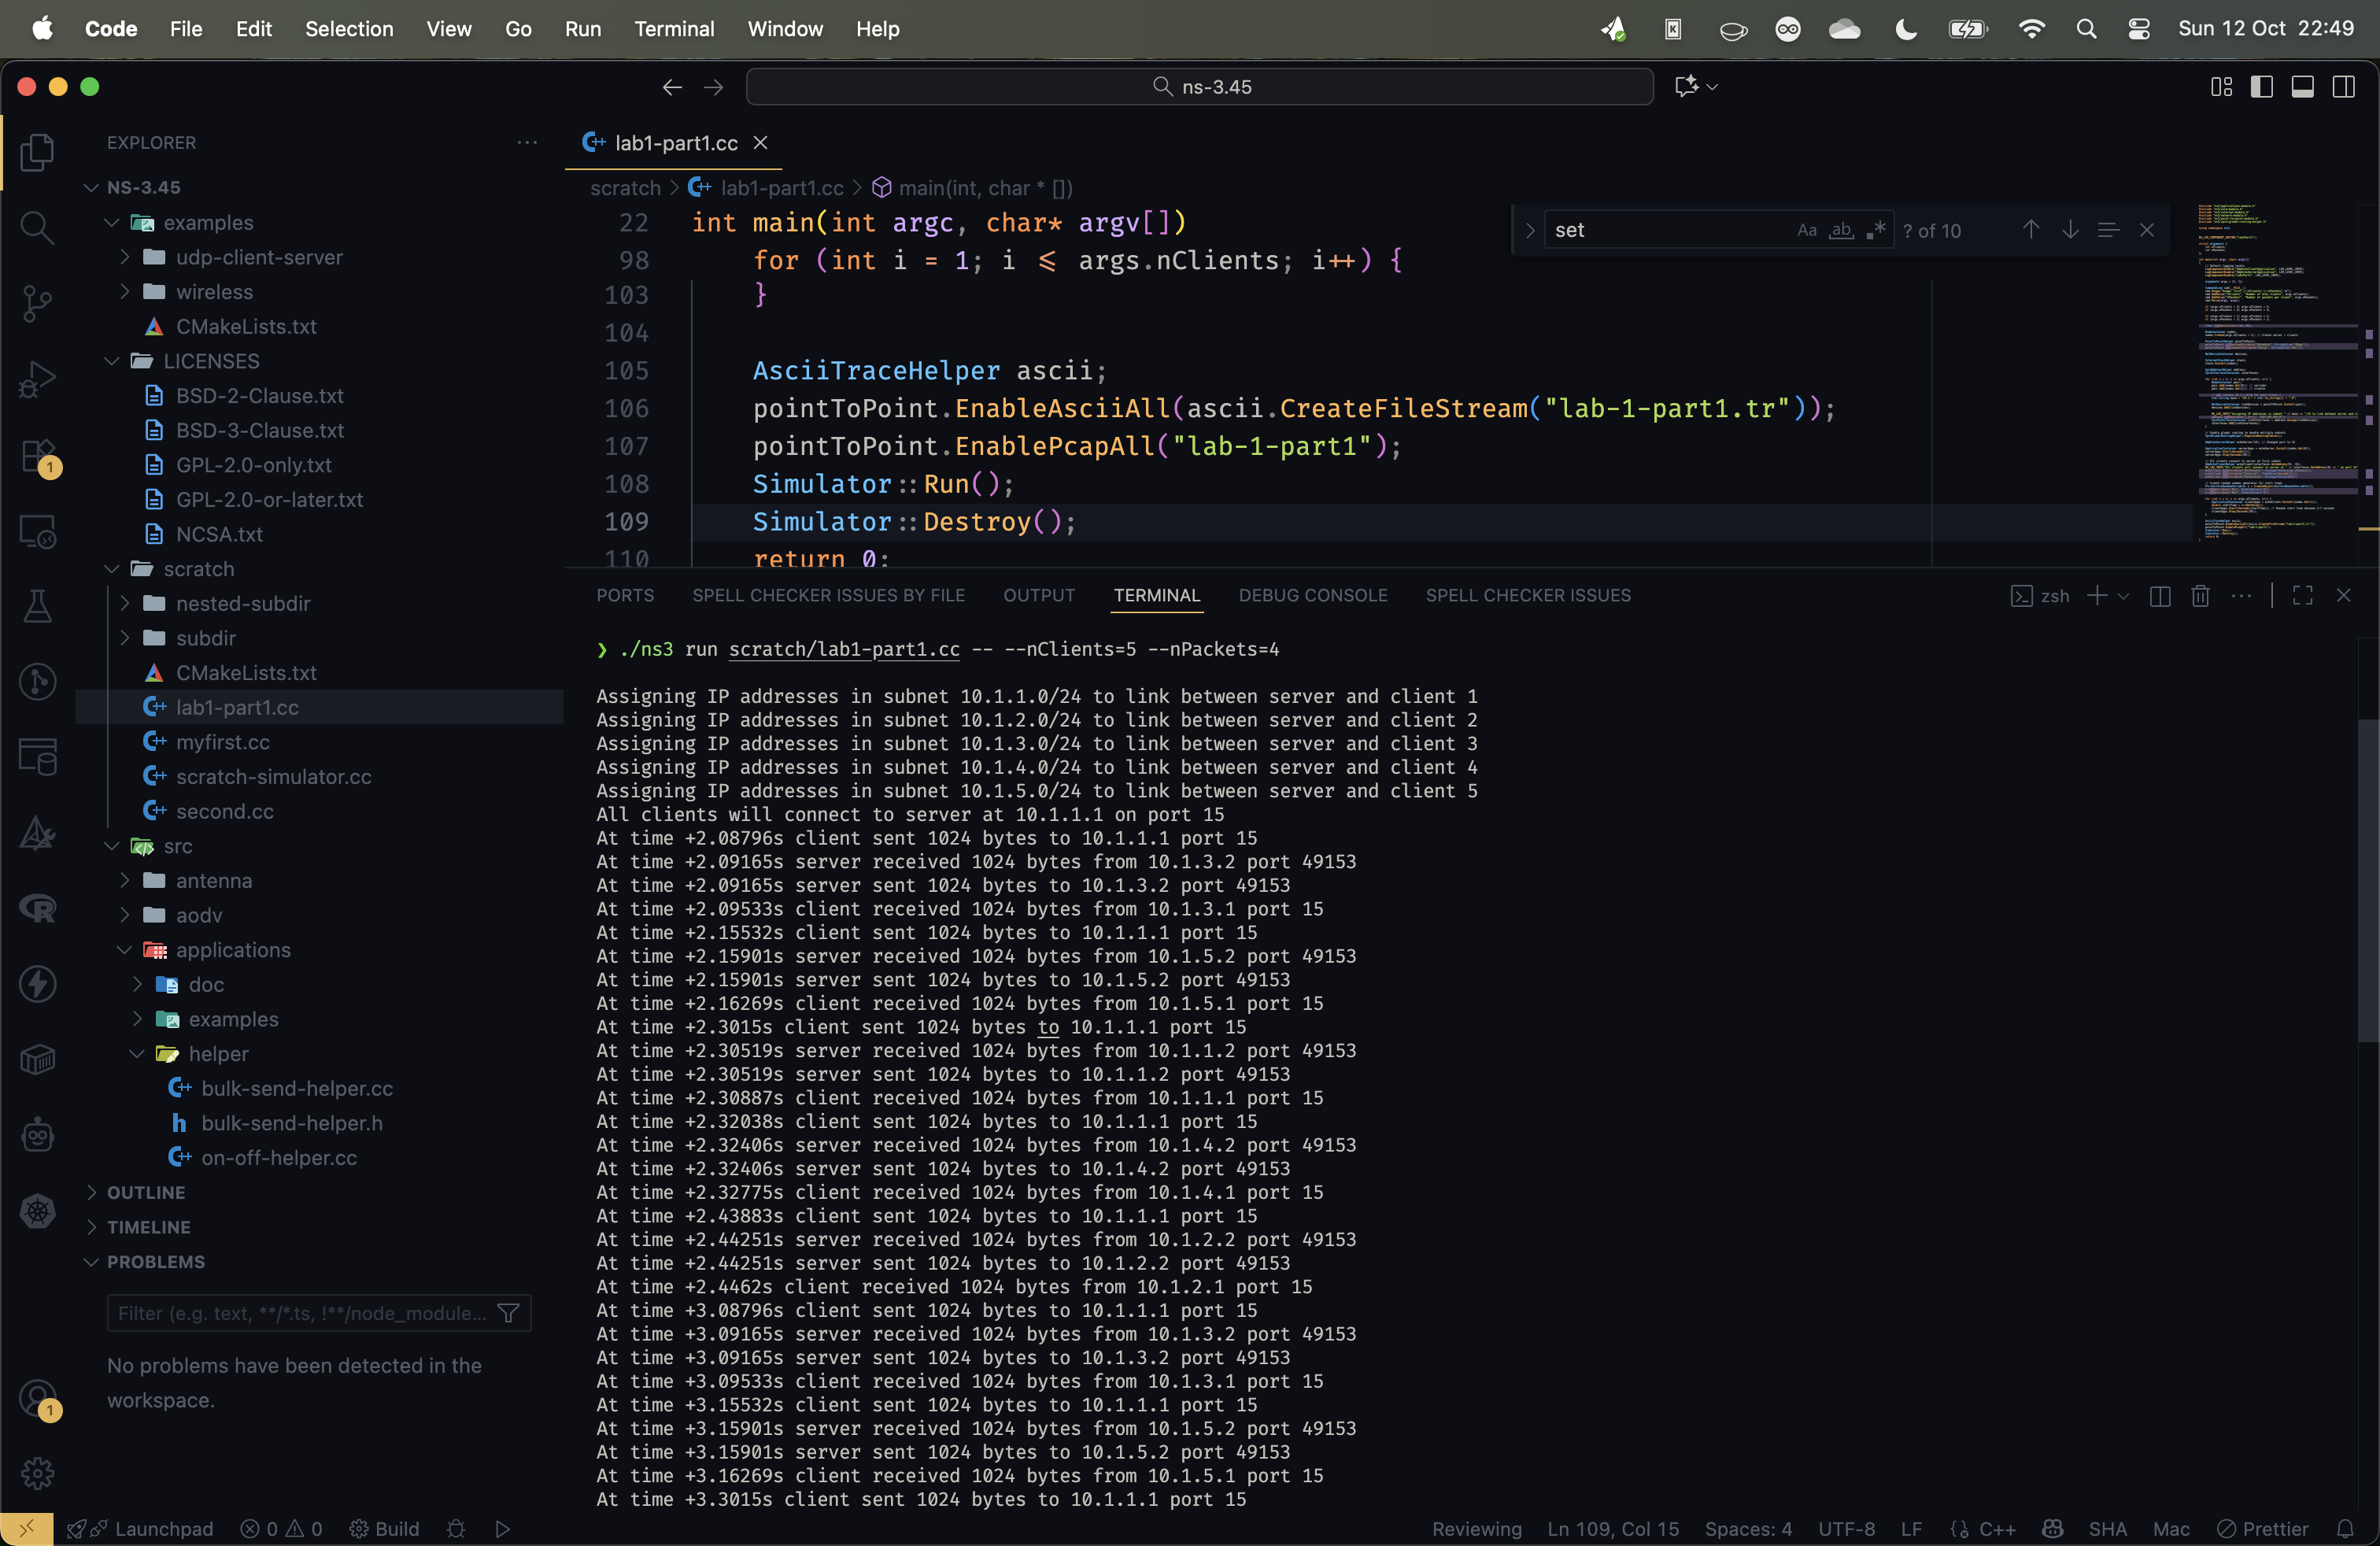
\includegraphics[width=1\textwidth]{lab1_exec_5_4.png}
    \caption{Execução da simulação da topologia em estrela com 5 clientes e 4 pacotes UDP enviados por cada cliente.}
    \label{fig:star_topology}
\end{figure}

\subsection{Redes ethernet}

A segunda parte do trabalho envolveu a criação de uma rede Ethernet simples usando a tecnologia CSMA. A figura \ref{fig:ethernet_topology} mostra a configuração da rede Ethernet, onde vários nós estão conectados a um canal CSMA. Além disto nesta configuração, cada extremidade da rede CSMA é conectada ponto a ponto com um nó. Nesta configuração o cliente UDP é instalado no nó ponto a ponto mais a esquerda na rede 10.1.1.0/24 e o servidor UDP é instalado no nó ponto a ponto mais a direita na rede 10.1.3.0/24.

\begin{figure}
    \centering
    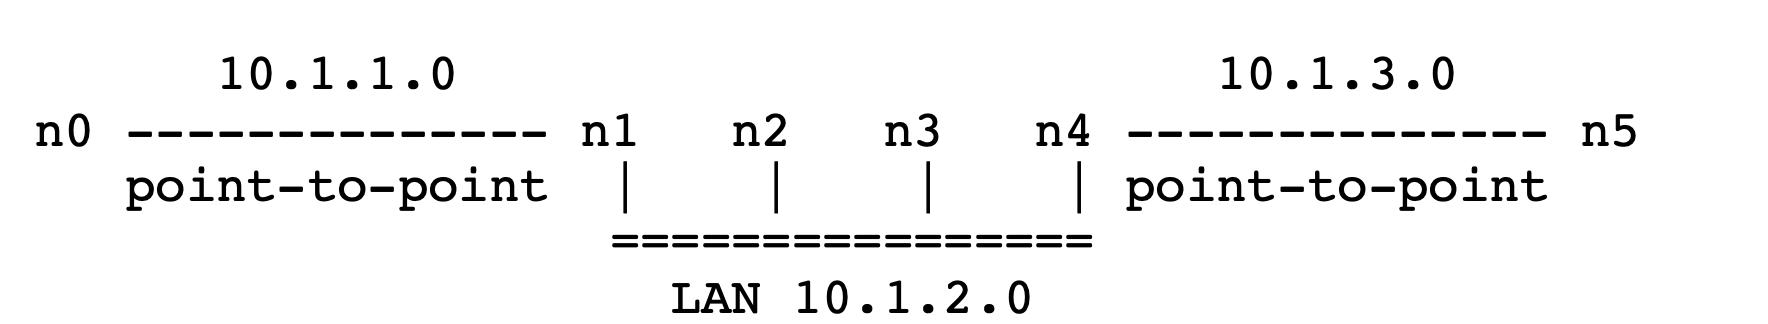
\includegraphics[width=1\textwidth]{layout_csma.png}
    \caption{Execução da simulação da rede Ethernet com 4 nós CSMA e 2 nós ponto a ponto nas extremidades.}
    \label{fig:ethernet_topology}
\end{figure}

A implementação que seguiu foi baseada no código exemplo \texttt{second.cc} fornecido pelo NS3. Após a modificação do código, a simulação foi executada com sucesso, conforme ilustrado na figura \ref{fig:ethernet_simulation}. A saída do terminal mostra que os pacotes foram enviados e recebidos corretamente, indicando que a rede CSMA está funcionando conforme o esperado.

\begin{figure}
  \centering
  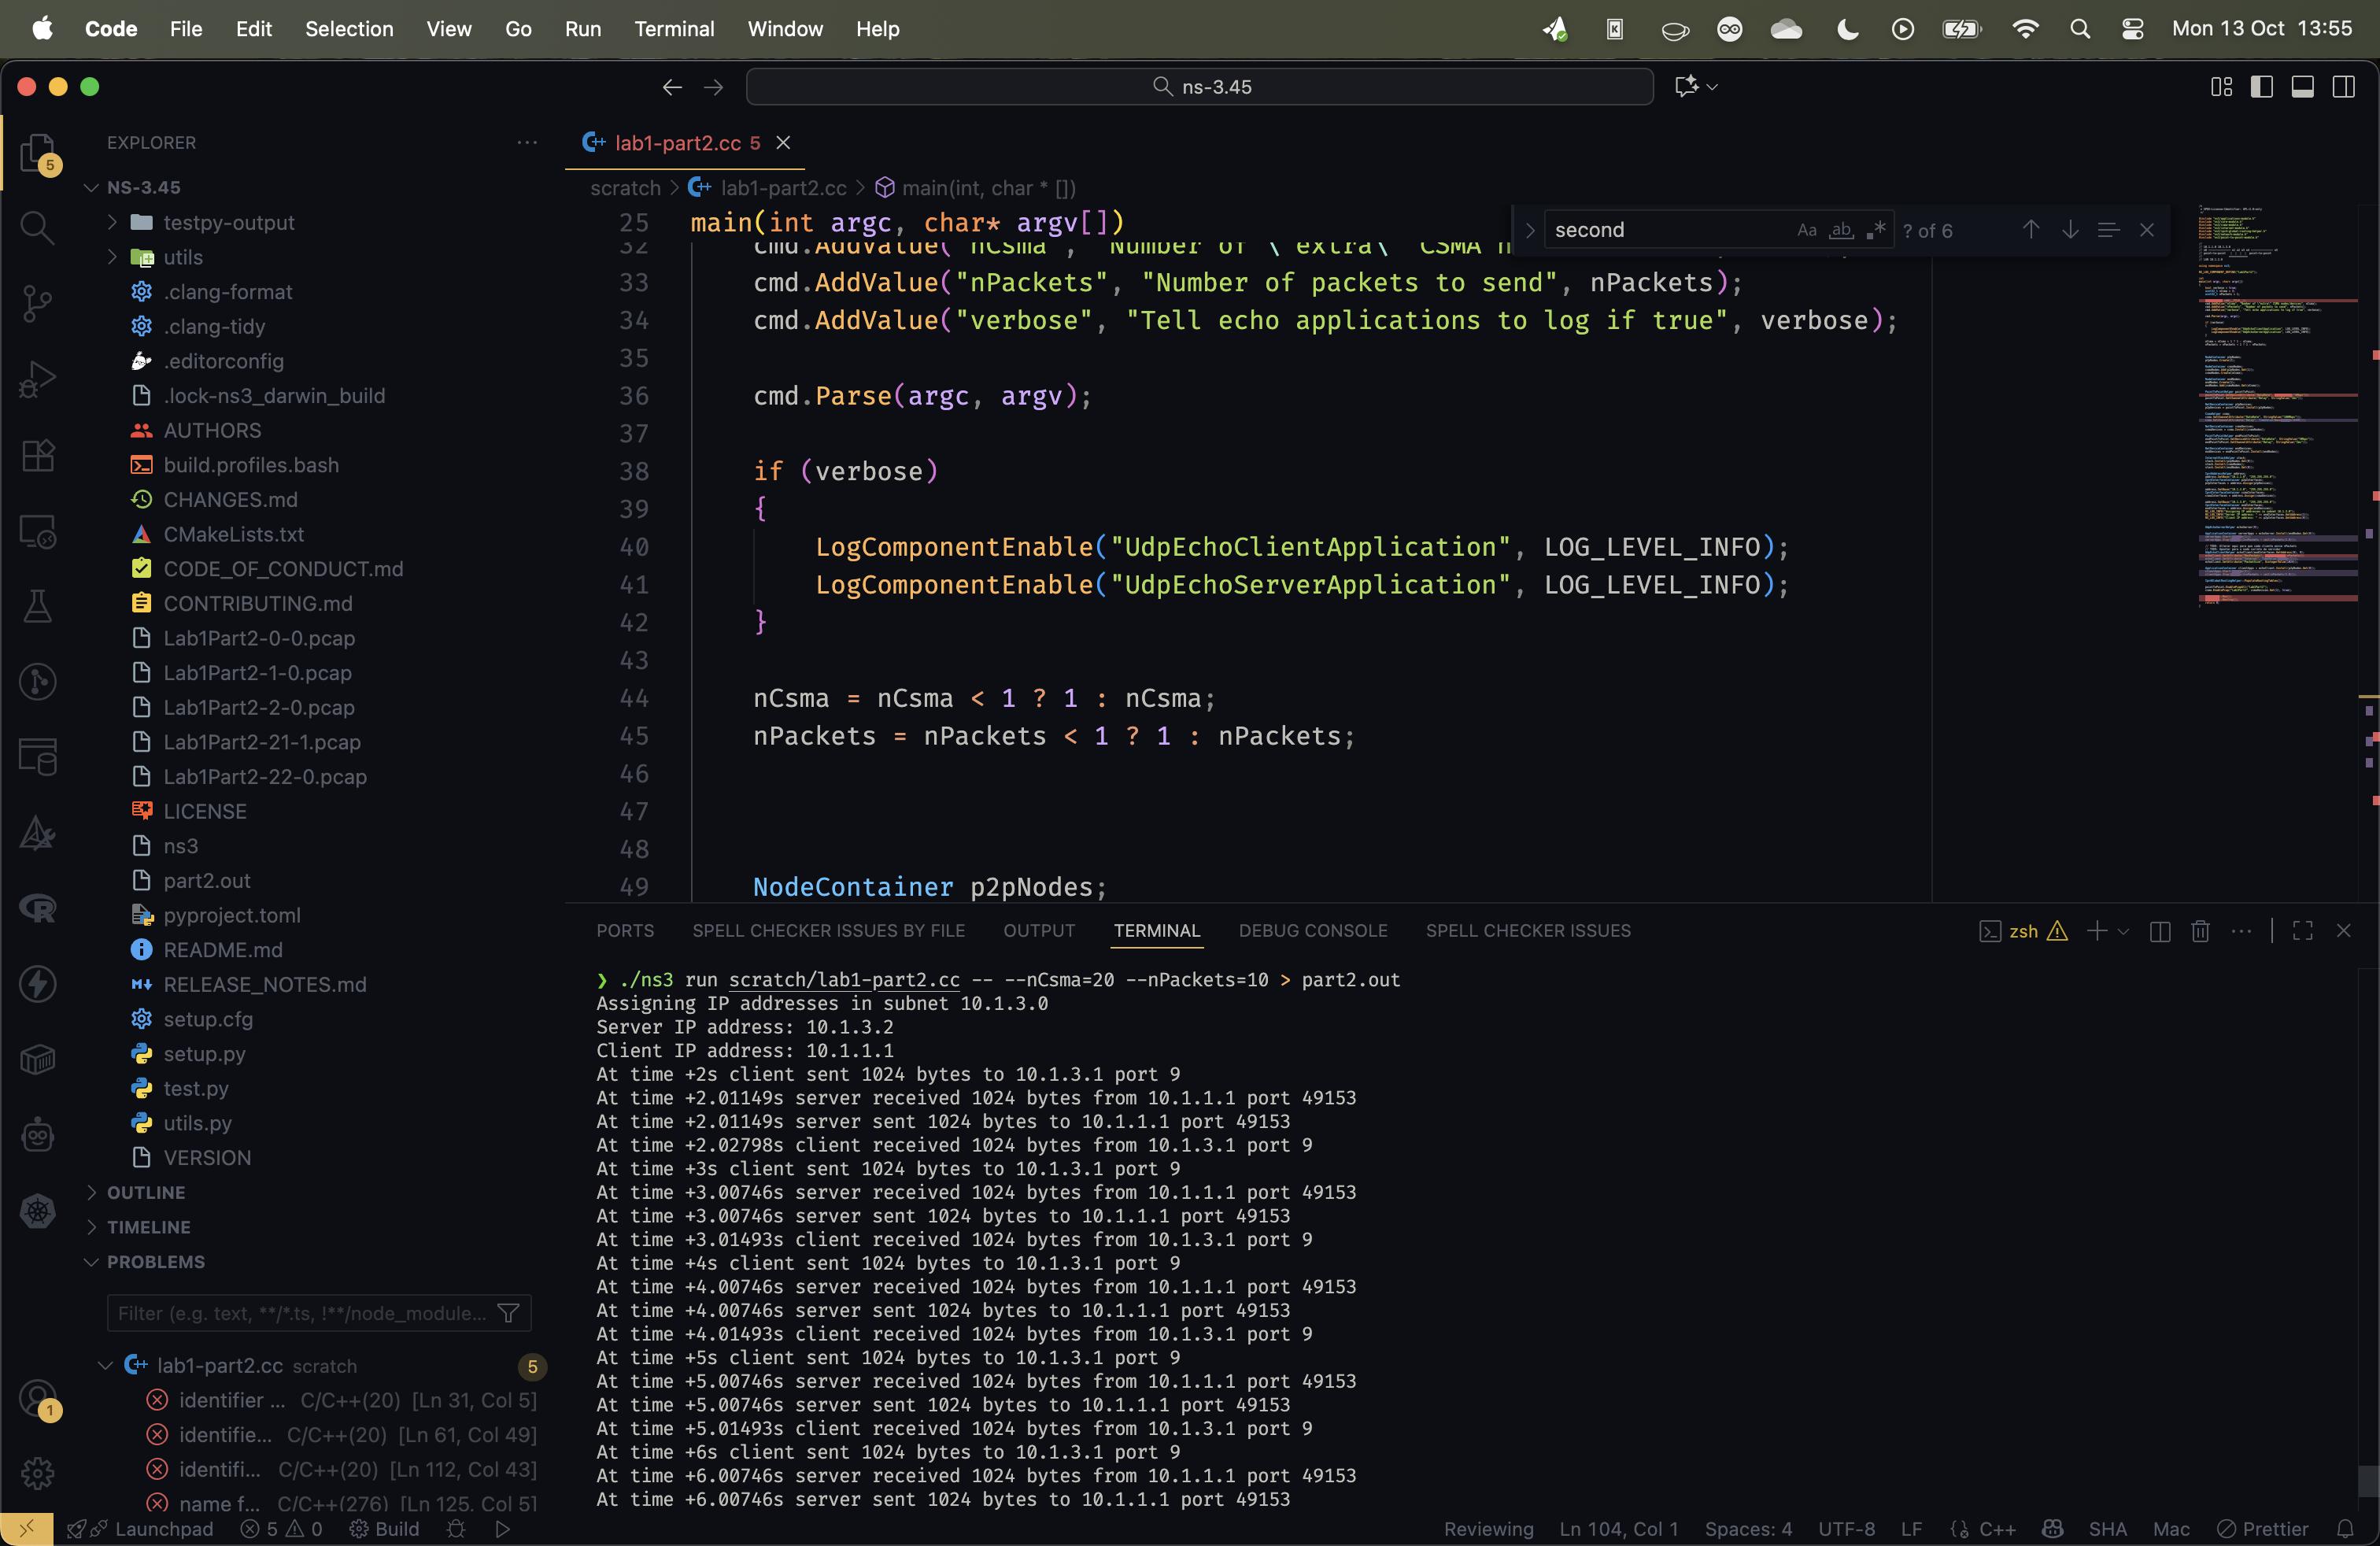
\includegraphics[width=1\textwidth]{run_csma.png}
  \caption{Execução da simulação da rede Ethernet com 20 nós CSMA e 2 nós ponto a ponto nas extremidades. Foram também enviados 10 pacotes UDP na simulação.}
  \label{fig:ethernet_simulation}
\end{figure}

Contudo, o envio e confirmação de recebimento do primeiro pacote UDP demorou mais do que os demais. Isto foi posteriormente confirmado pela análise de um dos arquivos \texttt{pcap} gerados pela simulação, que pode ser visualizado usando a ferramenta Wireshark. A figura \ref{fig:wireshark_analysis} mostra a análise do tráfego de rede capturado e nela é possível observar algumas comunicações ARP (Address Resolution Protocol) que ocorreram antes do envio do primeiro pacote UDP. Essas comunicações ARP são necessárias para que os nós possam resolver as rotas para os endereços IP dos destinatários, o que explica a demora inicial.

\begin{figure}
  \centering
  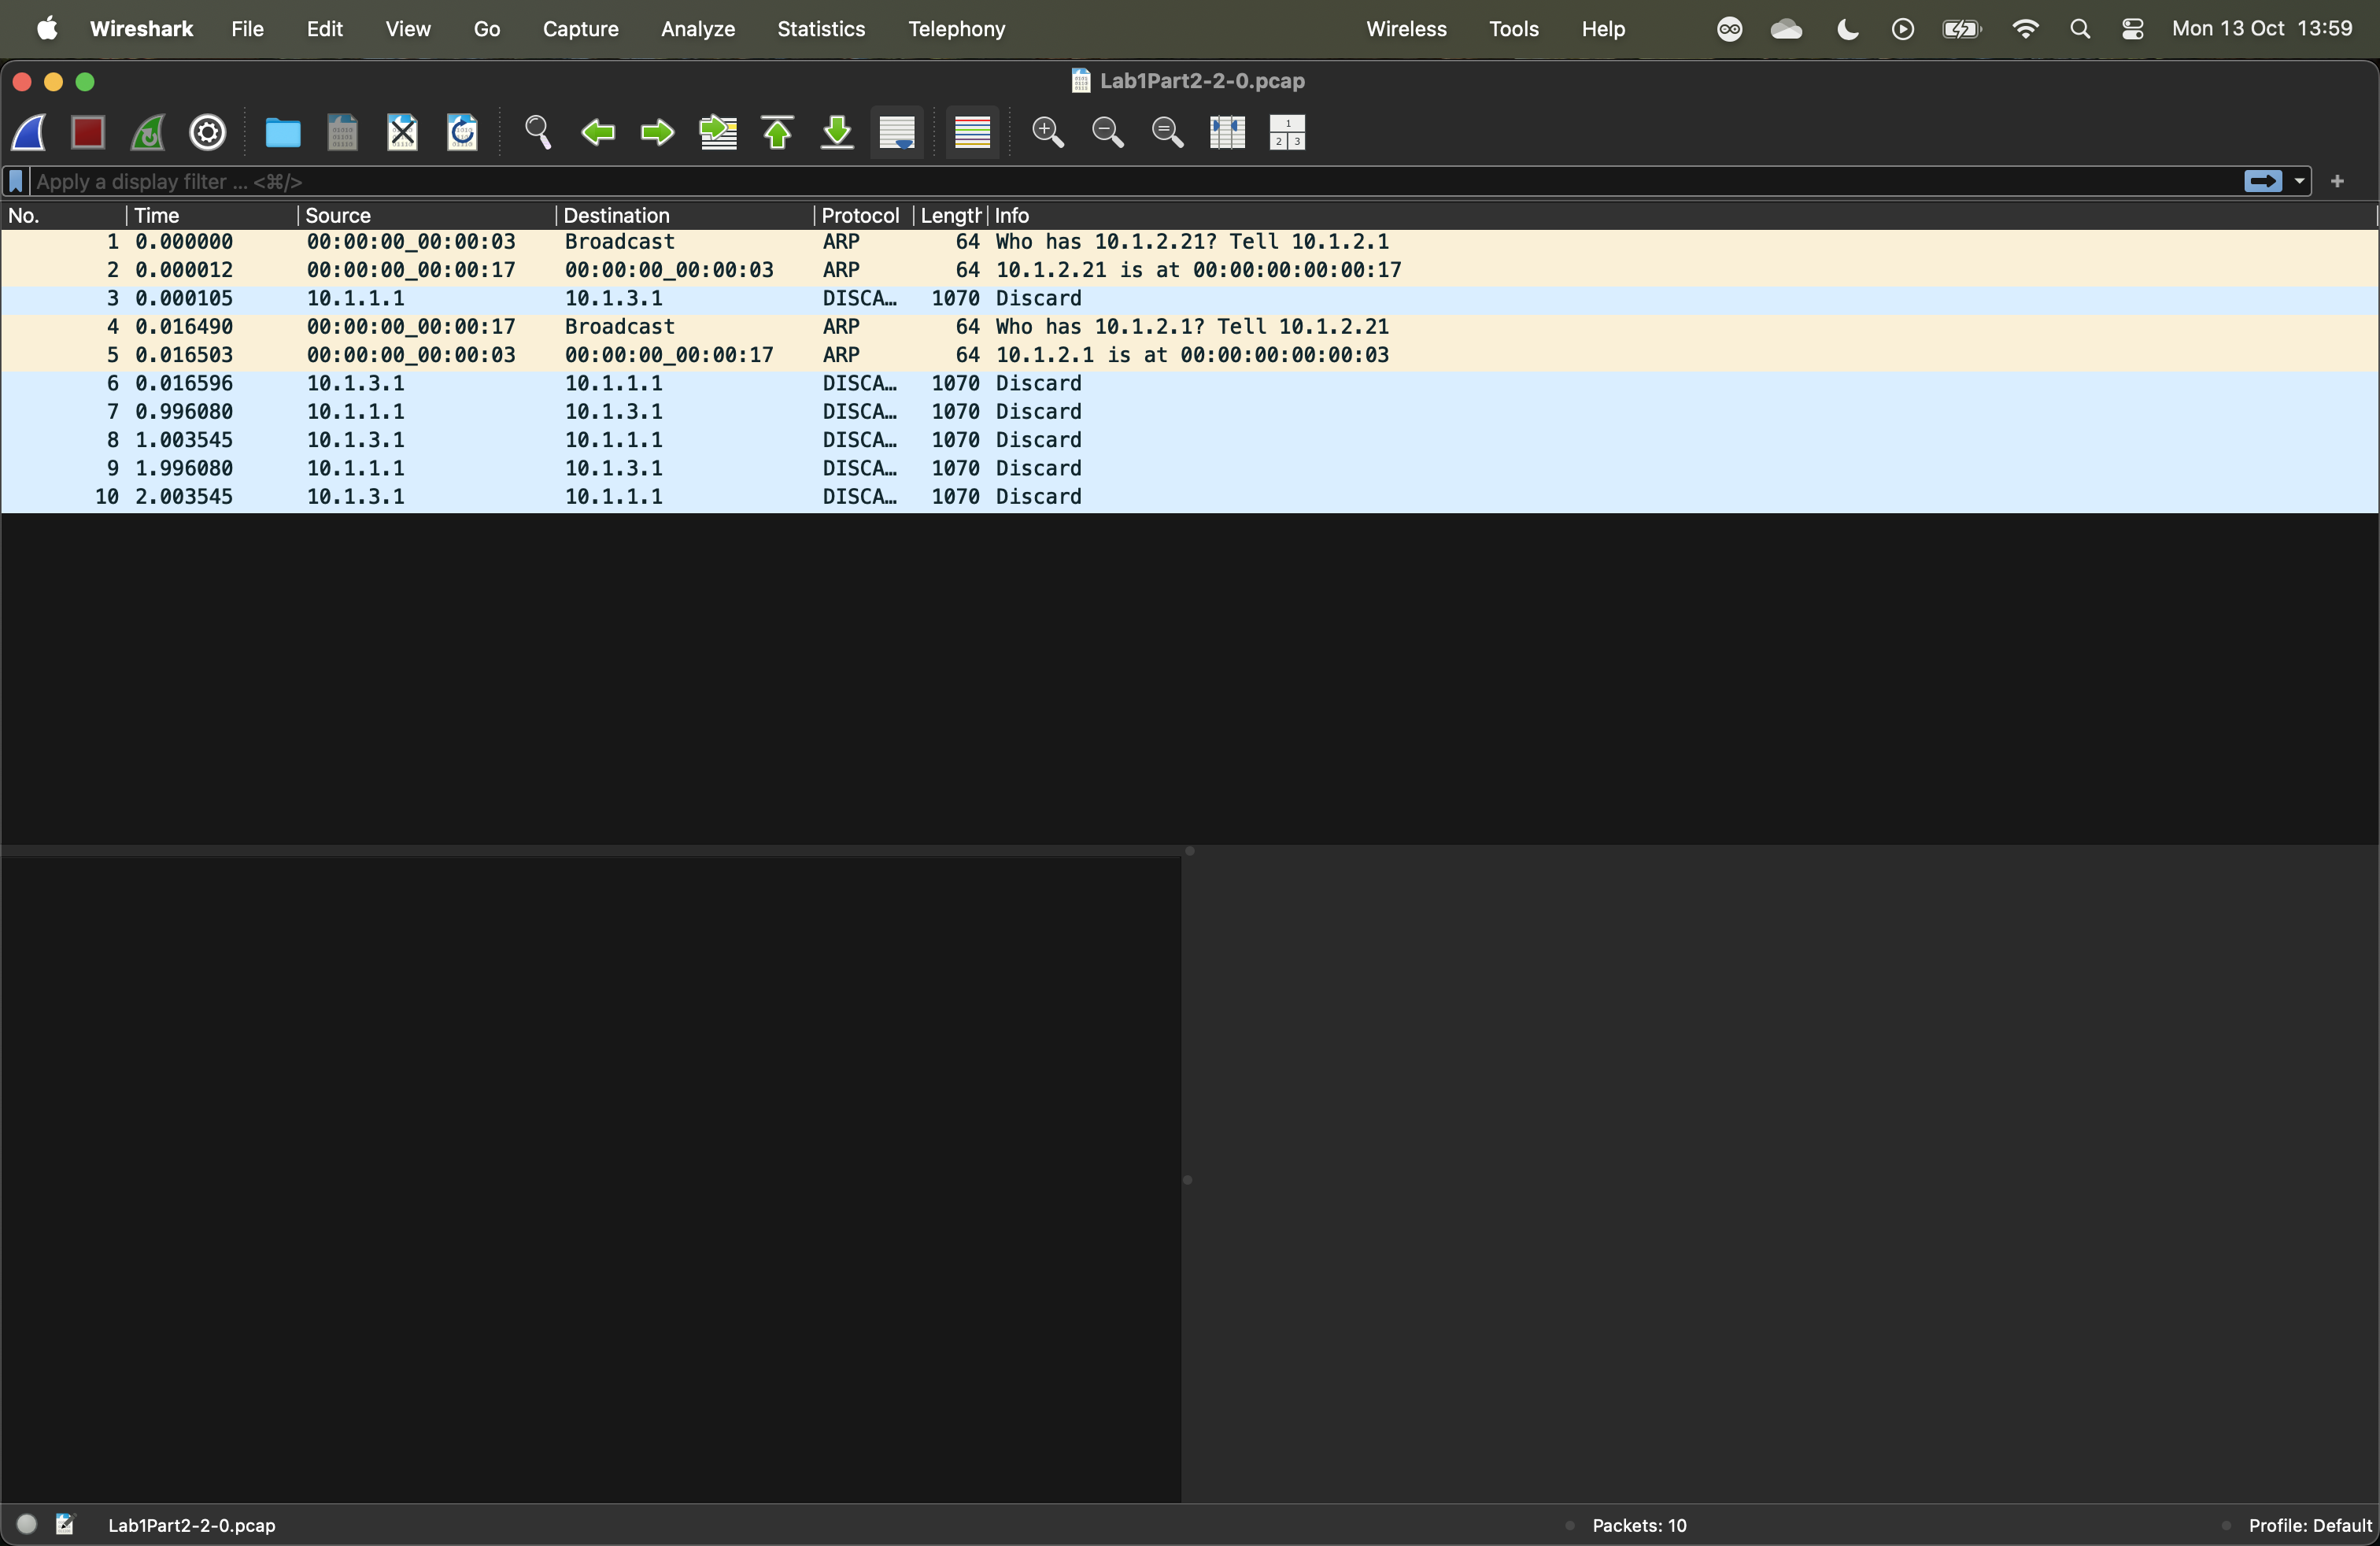
\includegraphics[width=1\textwidth]{wireshark_csma.png}
  \caption{Análise do tráfego de rede capturado usando Wireshark. A imagem mostra as comunicações ARP que ocorreram antes do envio do primeiro pacote UDP, explicando a demora inicial.}
  \label{fig:wireshark_analysis}
\end{figure}

\subsection{Redes sem fio}

A terceira parte do trabalho envolveu a criação de uma rede sem fio utilizando o NS3. A figura \ref{fig:wireless_topology} ilustra a configuração da rede sem fio, onde vários nós estão conectados a um ponto de acesso (AP) que liga a outro nó ponto a ponto que também é um AP para outra rede com nWifi estações sem fio. No exemplo da ilustração um cliente UDP é instalado no nó sem fio mais a esquerda na rede 10.1.3.0/24, e o servidor UDP é instalado no nó sem fio mais a direita na rede 10.1.2.0/24.

\begin{figure}
  \centering
  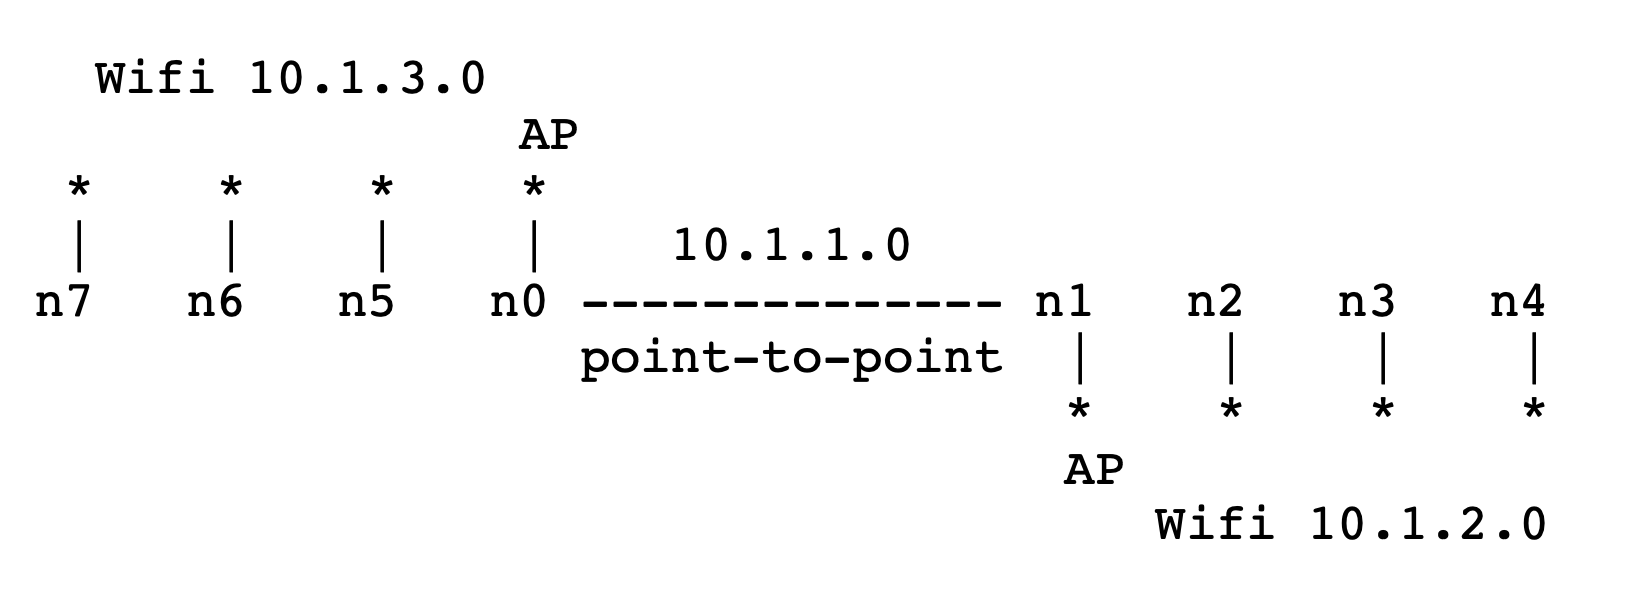
\includegraphics[width=1\textwidth]{wireless_topology.png}
  \caption{Execução da simulação da rede sem fio com 4 nós clientes e 1 ponto de acesso (AP).}
  \label{fig:wireless_topology}
\end{figure}

A implementação foi baseada no terceiro exemplo \texttt{third.cc} fornecido pelo NS3 \cite{ns3_tutorial}. Após a modificação do código, a simulação foi executada com sucesso, conforme ilustrado na figura \ref{fig:wireless_simulation}. A saída do terminal mostra que os pacotes foram enviados e recebidos corretamente, indicando que a rede sem fio está funcionando conforme o esperado. Além disso, nota-se que os tempos de transmissão e recepção dos pacotes são aleatórios. Isso pode ser consequência do tempo de transmissão variar devido a fatores como interferência, distância do ponto de acesso e condições do canal sem fio. O que também explica a ausência de uma configuração da largura de banda dos canais sem fio, uma vez que ela deve ser adaptativa as condições do ambiente.

\begin{figure}
  \centering
  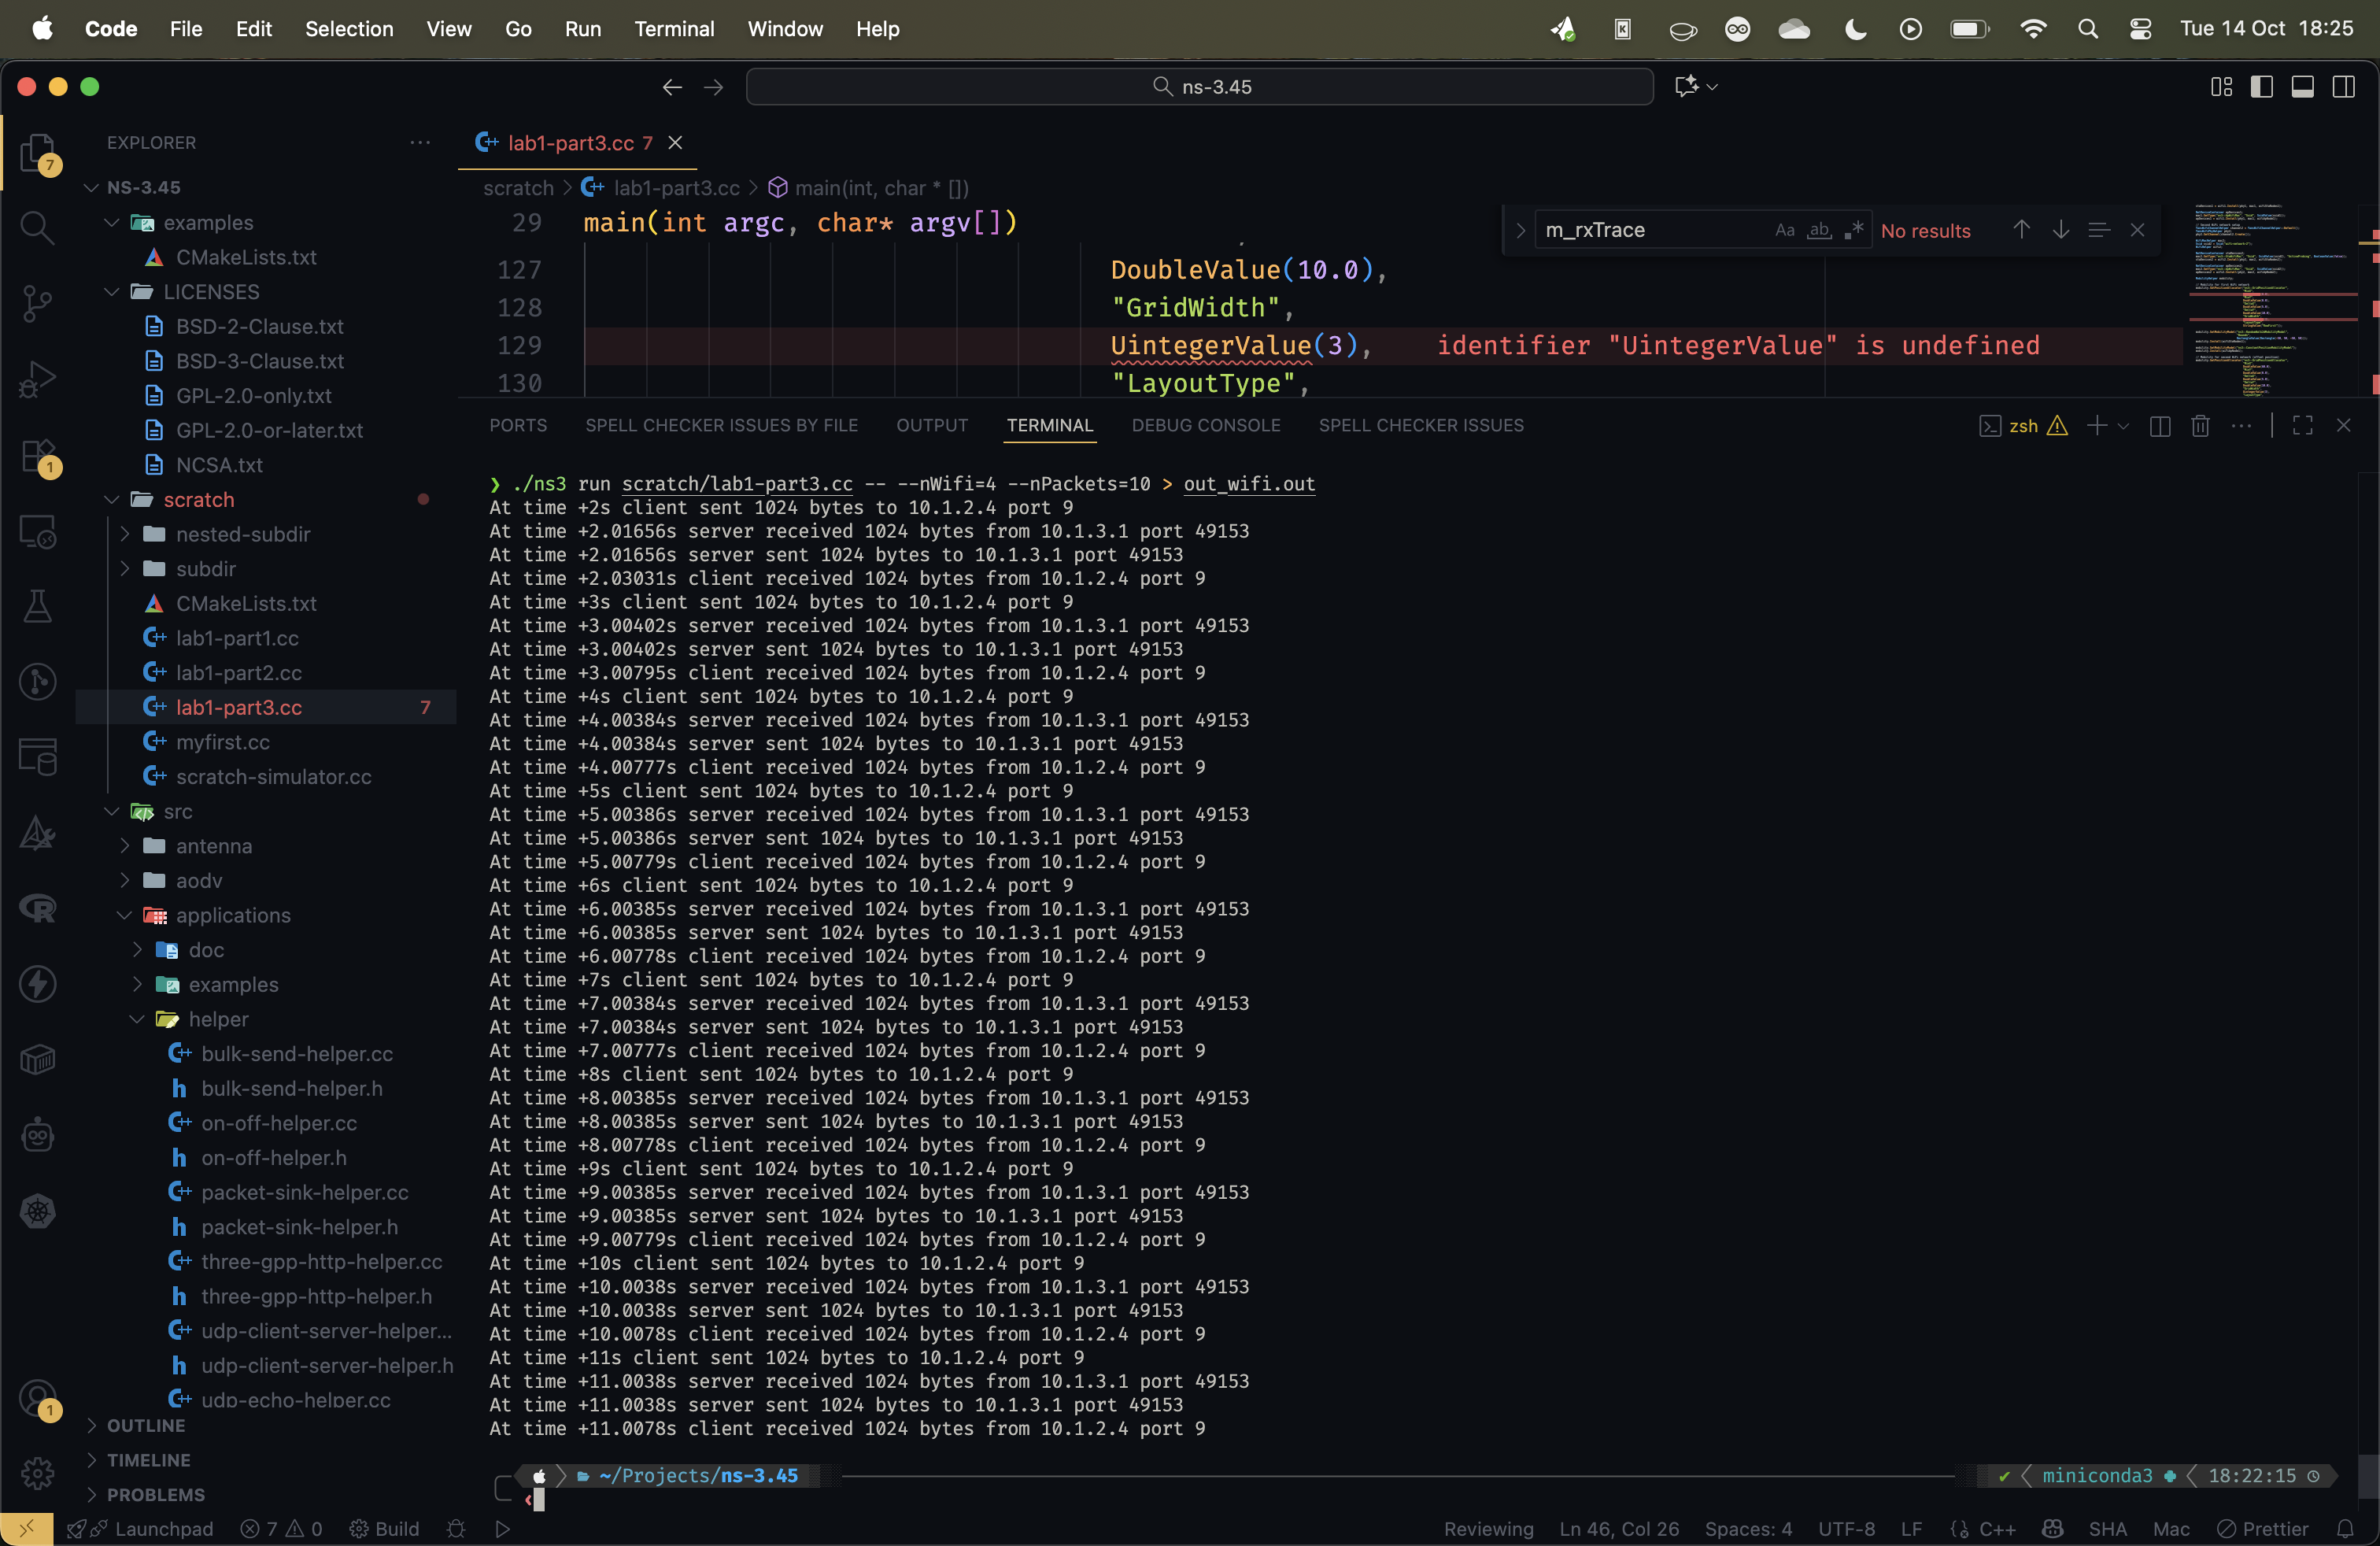
\includegraphics[width=1\textwidth]{run_wifi_4_10.png}
  \caption{Execução da simulação da rede sem fio com 4 nós clientes e 1 ponto de acesso (AP). Foram também enviados 10 pacotes UDP na simulação.}
  \label{fig:wireless_simulation}
\end{figure}

\section{Conclusão}

A execução deste trabalho foi um sucesso, mesmo que incompleta devido a dificuldade para configuração e geração de gráficos por meio da ferramenta de trace do NS3. Contudo, considero que a experiência adiquirida com uma plataforma de desenho e simulação de redes é muito valiosa para a formação acadêmica e profissional em engenharia de sistemas. A prática com o NS3 proporcionou uma compreensão mais profunda dos conceitos de redes de computadores, como topologias, protocolos e comunicação entre nós e diferenças entre diferentes meios de comunicação, como redes cabeadas e sem fio. 

Para trabalhos futuros, pretendo explorar mais a fundo as capacidades do NS3, incluindo a geração de gráficos e análises mais detalhadas dos resultados das simulações. Além disso, quero investigar maneiras de fazer visualizações mais intuitivas das topologias e dos dados fornecidos pelas simulações, o que pode enriquecer ainda mais a apresentação dos resultados. 

\clearpage
\addcontentsline{toc}{section}{Referências}
\bibliographystyle{plain}
\bibliography{references}

\end{document}